
\section{Introduction}
\subsection{Introduction}
\begin{frame}{Introduction}
Article présenté :\\
\alert{\textit{Tiny Web Serices: Design and Implementation of Interoperable and Evolvable Sensor Networks}}\\
Auteurs :\\
Nissanka B. \textsc{Priyantha}, Aman \textsc{Kansal}, Mishel \textsc{Goraczko} et Feng \textsc{Zhao}
\begin{itemize}
\item Sujet : solution pour un réseau de capteurs évolutif et interopérable basé sur les web services
\item Idée : couche applicative commune et bien connue pour différents capteurs $\Rightarrow$ réseau évolutif accessible à différentes applications. \\Nouvelle application: réutilisation de capteurs déjà en place
\end{itemize}
Toutes les figures proviennent de cet article.
\end{frame}

\begin{frame}{Exemple de nouvelle application}
Ajout d'une application de gestion de l'énergie basée sur des capteurs pour la sécurité et pour le système d'alerte médicale: 
\begin{figure}
  \centering
  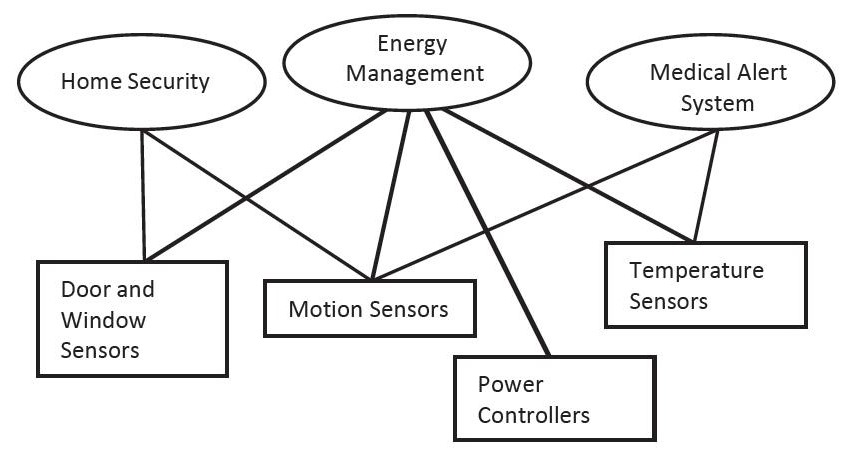
\includegraphics[scale=0.4]{figures/exemple.jpg}
  \caption{Exemple de réseau}
 \end{figure} 
\end{frame}


\begin{frame}{Composants}
2 fonctionnalités clés:
\begin{itemize}
\item Données structurées : compréhension des applications (exemple XML)
\item Accès aux fonctionnalités par appel de fonction : description des fonctionnalités du capteur accessibles au programmeur
\end{itemize}
Ces fonctionnalités existent déjà pour se connecter à Internet par exemple et sont disponibles au travers des web services.\\ 
\begin{block}{Challenge}
Minimiser le coût en ressources : standards non optimisés pour des appareils de faible puissance
\end{block}
\end{frame}

\begin{frame}{But}
\begin{itemize}
\item Estimation du coût en ressources
\item Identification des choix de design qui minimisent ce coût
\item Analyse de l'impact négatif de ces choix 
\end{itemize}
\begin{block}{Problématique}
Peut-on accepter les impacts négatifs de cette approche?
\end{block}
\end{frame}

\begin{frame}{Simulation d'un capteur à ressources limitées}
Caractéristiques du capteur prototype:
\begin{itemize}
\item Processeur MSP430 à 6Mhz
\item Mémoire ROM de 48k
\item Consommation énergétique équivalente à celle de la plupart des capteurs de faible puissance
\item Interface radio IEEE 802.15.4, vitesse de transfert maximale 250kbps
\end{itemize}
\begin{figure}
  \centering
  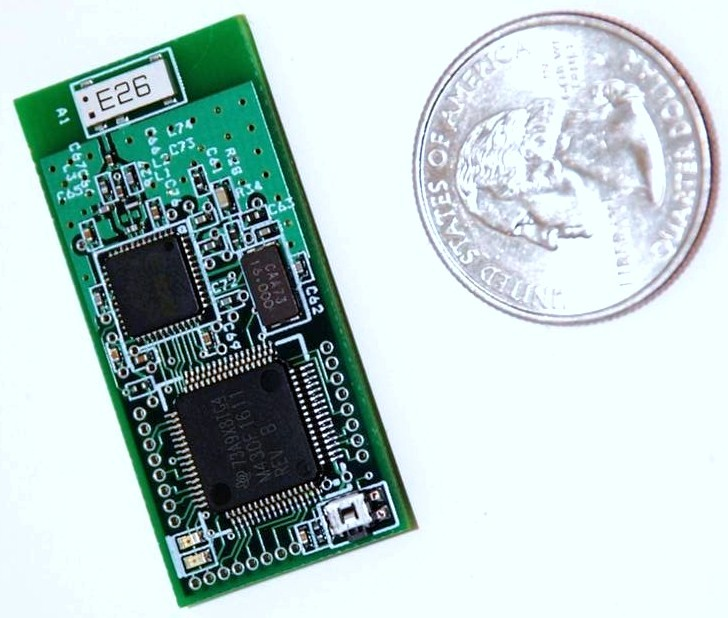
\includegraphics[scale=0.15]{figures/tws08-000.jpg}
  \caption{Capteur sans fil expérimental}
 \end{figure} 
\end{frame}

\begin{frame}{Travaux liés}
Travaux utiles pour réaliser cette étude :
\begin{itemize}
\item XML sur des capteurs : format standard de données
\item Services web embarqués 
\item Implémentation de web services : Devices Profile for Web Services (DPWS), utilisation de passerelles.
\item Couche réseau : nécessaire pour supporter la couche applicative
\item WS-Eventing : support du sleep mode et duty cycle
\item XML compression : gain de mémoire
\end{itemize}
\begin{block}{Différence}
Contrainte en ressources due aux appareils considérés
\end{block}
\end{frame}

\section{Web services}
\subsection{Web services}
\begin{frame}{Web services}
\framesubtitle{Définition}
Mécanisme pour utiliser des ressources à distance de la même façon que des ressources locales.\\
Les standards définissent 2 composants clés:
\begin{itemize}
\item \textit{Ports} : méthodes disponibles sur le serveur  
\item \textit{Bindings}: protocoles réseaux supportés pour chaque méthode
\end{itemize}
Ces 2 composants sont définis via le Web Services Description Language (WSDL), les spécifications du web service est référencé par sa description WSDL.
\end{frame}

\begin{frame}
\frametitle{Exemple WSDL}
\framesubtitle{Méthode}
\begin{exampleblock}{Déclaration d'une méthode}
\verbatiminput{wsdlEx.xml}
\end{exampleblock}
\end{frame}

\begin{frame}
\frametitle{Exemple WSDL}
\framesubtitle{Binding}
\begin{exampleblock}{binding à HTTP}
\verbatiminput{bindingEx.xml}
\end{exampleblock}
\end{frame}

\begin{frame}
\frametitle{Exemple WSDL}
\framesubtitle{Requête}
\begin{exampleblock}{\texttt{SetTemperature(25)} par URL}
\texttt{http://192.168.1.4/setTemp?temp=25}
\end{exampleblock}
\end{frame}

\begin{frame}{Avantages}
Couche applicative:
\begin{itemize}
\item Partage des ressources de manière très flexible %: meilleure performance des applications existantes, déploiement de nouvelles applications sans forcément de nouveaux capteurs.
\item Facilité de programmation %: la description WSDL peut facilement être traduite en un langage haut niveau et le programmeur voit uniquement un objet avec les méthodes appropriées.
\item Facilité d’intégration dans les réseaux d’entreprise %: il existe déjà beaucoup d’applications réseau basées sur les web services. Si les capteurs disposent d’interfaces similaires, alors les données physiques générées peuvent être utilisées pour donner de nouvelles possibilités aux applications existantes.
\item Suppression des gateways (passerelles)% : la traduction des formats de messages  custom  de chaque fabricant n’est plus nécessaire.
\end{itemize}
\vspace{5mm}
Couche réseau IP:
\begin{itemize}
\item facilité de gestion de réseau
\item utilisation de DHCP pour l’allocation d’adresses
\item valide pour différentes couches physiques
\end{itemize}
\end{frame}
%Inconvénient déplacé sur slide but

